% !TEX root = ../main.tex

In preparation for the 2015 DARPA Robotics Challenge (DRC) Finals, Team ViGIR, as well as many other teams, developed an approach to high-level robot control \cite{Philipp2015MSc}.
However, these approaches relied on experts developing scripted behaviors or, in our case, manually designing state-machine-based controllers.
In addition, there was no guarantee that the resulting high-level behaviors were correct with respect to the tasks at hand.
Moreover, many participants observed that such approaches were fragile in practice \cite{DRC-what-happened}.
Motivated by these shortcomings, and enabled by recent advances in the field of formal methods for robotics 
\cite{Vasu2013ICRA, Vasu2015TRO, JFRKG2012ICRA, Lignos2015AURO, Kavraki2015AAAI, Kavraki2015ICRA, Belta2014TAC, Fainekos2014ICRA, Dimos2014ICRA, Jon2015ICRA, Ben2015IJRR, Wolff2014ICRA, Ankur2015ISRR, Finucane2010IROS, Topcu2011RAM}, 
we present an approach for the synthesis of provably correct reactive high-level robot behavior and the 
automatic generation of the corresponding software implementation.

\begin{figure}[t]
\centering
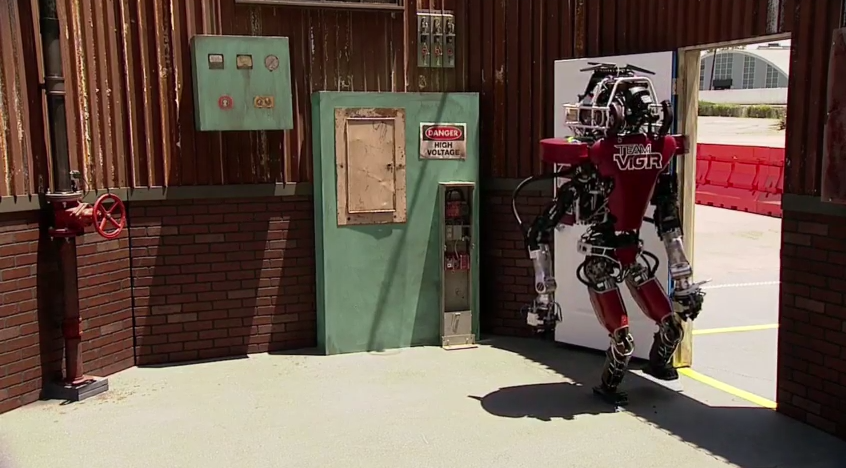
\includegraphics[width=0.99\columnwidth,clip]{./img/atlas_door_finals.png}
\caption{Team ViGIR's Atlas humanoid robot on the first day of the DRC Finals. (Photo credit: DARPA)
}
\label{Fig:AtlasDoorFinals}
\vspace{-10pt}
\end{figure}

\begin{myExample}\label{Ex:TurnValve}
	Consider the DRC task of walking to the valve and turning it (Fig. \ref{Fig:AtlasDoorFinals}).
	Carrying out this task involves steps such as object detection, footstep planning, manipulation, etc.
	These capabilities also differ from robot to robot.
	Ideally, a non-expert user should be able to specify such tasks in terms of the goals to be achieved, without having to worry about the details of how the robotic system will achieve them.
	Moreover, it would be advantageous if any failures that might occur during execution were automatically handled.
\end{myExample}

To this end, we automatically generate logic-based specifications from a higher level, multi-paradigm specification: a user-specified task and the description of the system's capabilities, which includes constraints such as action preconditions, and is set up \emph{a priori} by the system designers.
Furthermore, most approaches employing formal methods assume that the low-level system components that make up the high-level plan will work as expected, i.e., they never fail.
In this paper, we lift this assumption by formally accounting for the possibility of failure when executing the low-level components.
While there might be no way to recover from such a failure, we can still achieve \emph{graceful degradation}.
That is, we can formally specify the system's reaction to failure.

Finally, we bridge the gap between theoretical results and practice. 
Thus, we automatically generate the software implementation of a state machine that instantiates the synthesized mission plan by grounding it to the robotic system's capabilities.
The result is in an end-to-end approach.
We present and experimentally validate this approach in the context of a complex system, a Boston Dynamics Atlas humanoid robot (Fig. \ref{Fig:AtlasDoorFinals}) running the software that Team ViGIR developed for the DRC.
Note that the concepts are general and apply to different systems.
We have implemented and open-sourced the proposed approach as a collection of Robot Operating System (ROS \cite{ROS}) packages.

The rest of this paper is organized as follows.
In Section \ref{S:lit}, we compare our contributions to the state of the art.
In Section \ref{S:prelim}, we introduce Team ViGIR's approach to the DRC and Linear Temporal Logic (LTL).
In Section \ref{S:problem}, we state the technical problem that this paper addresses.
We present our approach in Sections \ref{S:abstraction} through \ref{S:synthesis} and summarize our ROS implementation in Section \ref{S:implementation}.
We present experimental demonstrations in Section \ref{S:experiments}.
We draw conclusions and propose future research directions in Section \ref{S:conclusion}.

%END